\chapter{Análisis de las imágenes}
\section{Análisis y factibilidad}
\noindent En este trabajo se propone realizar un análisis profundo de las mediciones existentes tomadas por el sensor, aplicando un corte de calidad a las imágenes que aumenta el número de eventos detectados por el programa, para así aumentar la estadística y mejorar la resolución con la que se calculan tanto el factor de Fano como la energía de creación electrón-hueco. %Sin embargo, aplicar este corte de calidad trae aparejado un sesgo en el conteo de carga de cada evento, tanto por defecto como por exceso, con lo cual es un efecto que debe corregirse.
En este sentido, es de gran importancia cuantificar el aumento en la estadística al modificar los parámetros usados en el programa de reconocimiento de clusters y así poder establecer la factibilidad de la mejora en el cálculo de las incertezas de los valores antes mencionados.\\
\indent El parámetro clave en este caso se llama \verb|EPIX|, y es un valor umbral, define a partir de qué cantidad de carga se cuenta o no como un píxel vacío. Por ejemplo, para \verb|EPIX = 0.5|, todos los píxeles con carga menor o igual $1$ se cuentan como píxeles vacíos, y los que tengan carga mayor a $1$ serán contabilizados normalmente, para \verb|EPIX = 1.5|, todos los píxeles con carga menor o igual a $2$ se cuentan como píxeles vacíos y los píxeles con carga mayor a $2$ se cuentan normalmente.\\
\indent En trabajos previos\cite{TesisKevin}, los valores obtenidos para el factor de Fano y energía de creación electrón-hueco, fueron calculados con un valor de \verb|EPIX = 0.5|. Se espera que al modificar este parámetro, el conteo de eventos varíe y que, en particular, aumente cuando el \verb|EPIX| aumenta. Esto se debe a que es muy común que se tenga un evento de interés, por ejemplo un cluster de $4$ píxeles de área y con una carga total de $180$ electrones, y alrededor de este se acumulen píxeles con cargas debidas a corrientes oscuras del sensor, de por ejemplo $1$ o $2$ electrones. En estos casos podría suceder que la conexión entre el cluster de interés y los píxeles con carga espuria se extiendan lo suficiente como para que el algoritmo reconozca un gran cluster con exceso de carga y sea filtrado dado que no cumple con los cortes de calidad impuestos. También podría suceder que estos píxeles con carga espuria conecten $2$ clusteres de interés, lo cual es un caso más extremo, dado que el algoritmo reconocería un único cluster de $\sim 360$ electrones, de forma que se perderían, no $1$, sino $2$ eventos que podrían aportar positivamente a la estadística. Al aplicar un umbral que elimine los píxeles con carga espuria que se amontonan y/o conectan con clusteres, el programa es capaz de diferenciar y contar los eventos correctamente.\\
\indent En la figura \ref{fig:ClusterPegoteado} se muestra un ejemplo de un evento de $174$ electrones, que es un evento de interés que el programa debería reconocer, y que hasta que no se eliminan los eventos de hasta $2$ electrones de la imagen, el programa lo identifica como un gran (y amorfo) cluster (imagen central, píxeles pintados de blanco). A la derecha la imagen con el cluster individualizado y reconocido correctamente por el algoritmo al eliminar la carga excedente.
\begin{figure}[H]
%Para modificar este plot hay que ir a /home/igna/Escritorio/Tesis2021/Figs/pys_para_plots y correr gradiente_filas_sensor.py Los datos los saca de /home/igna/Escritorio/Tesis2021/Figs/txts_para_plots y del archivo OHDU1/2/3/4_gradiente_filas_sensor.txt
%Esta imagen corresponde al set de imágenes que se procesaron con el parámetro B, y al primer cuadrante del sensor (que es el que mejor anda) Aclaro porque no lo aclaré en ningún otro lado
    \centering
    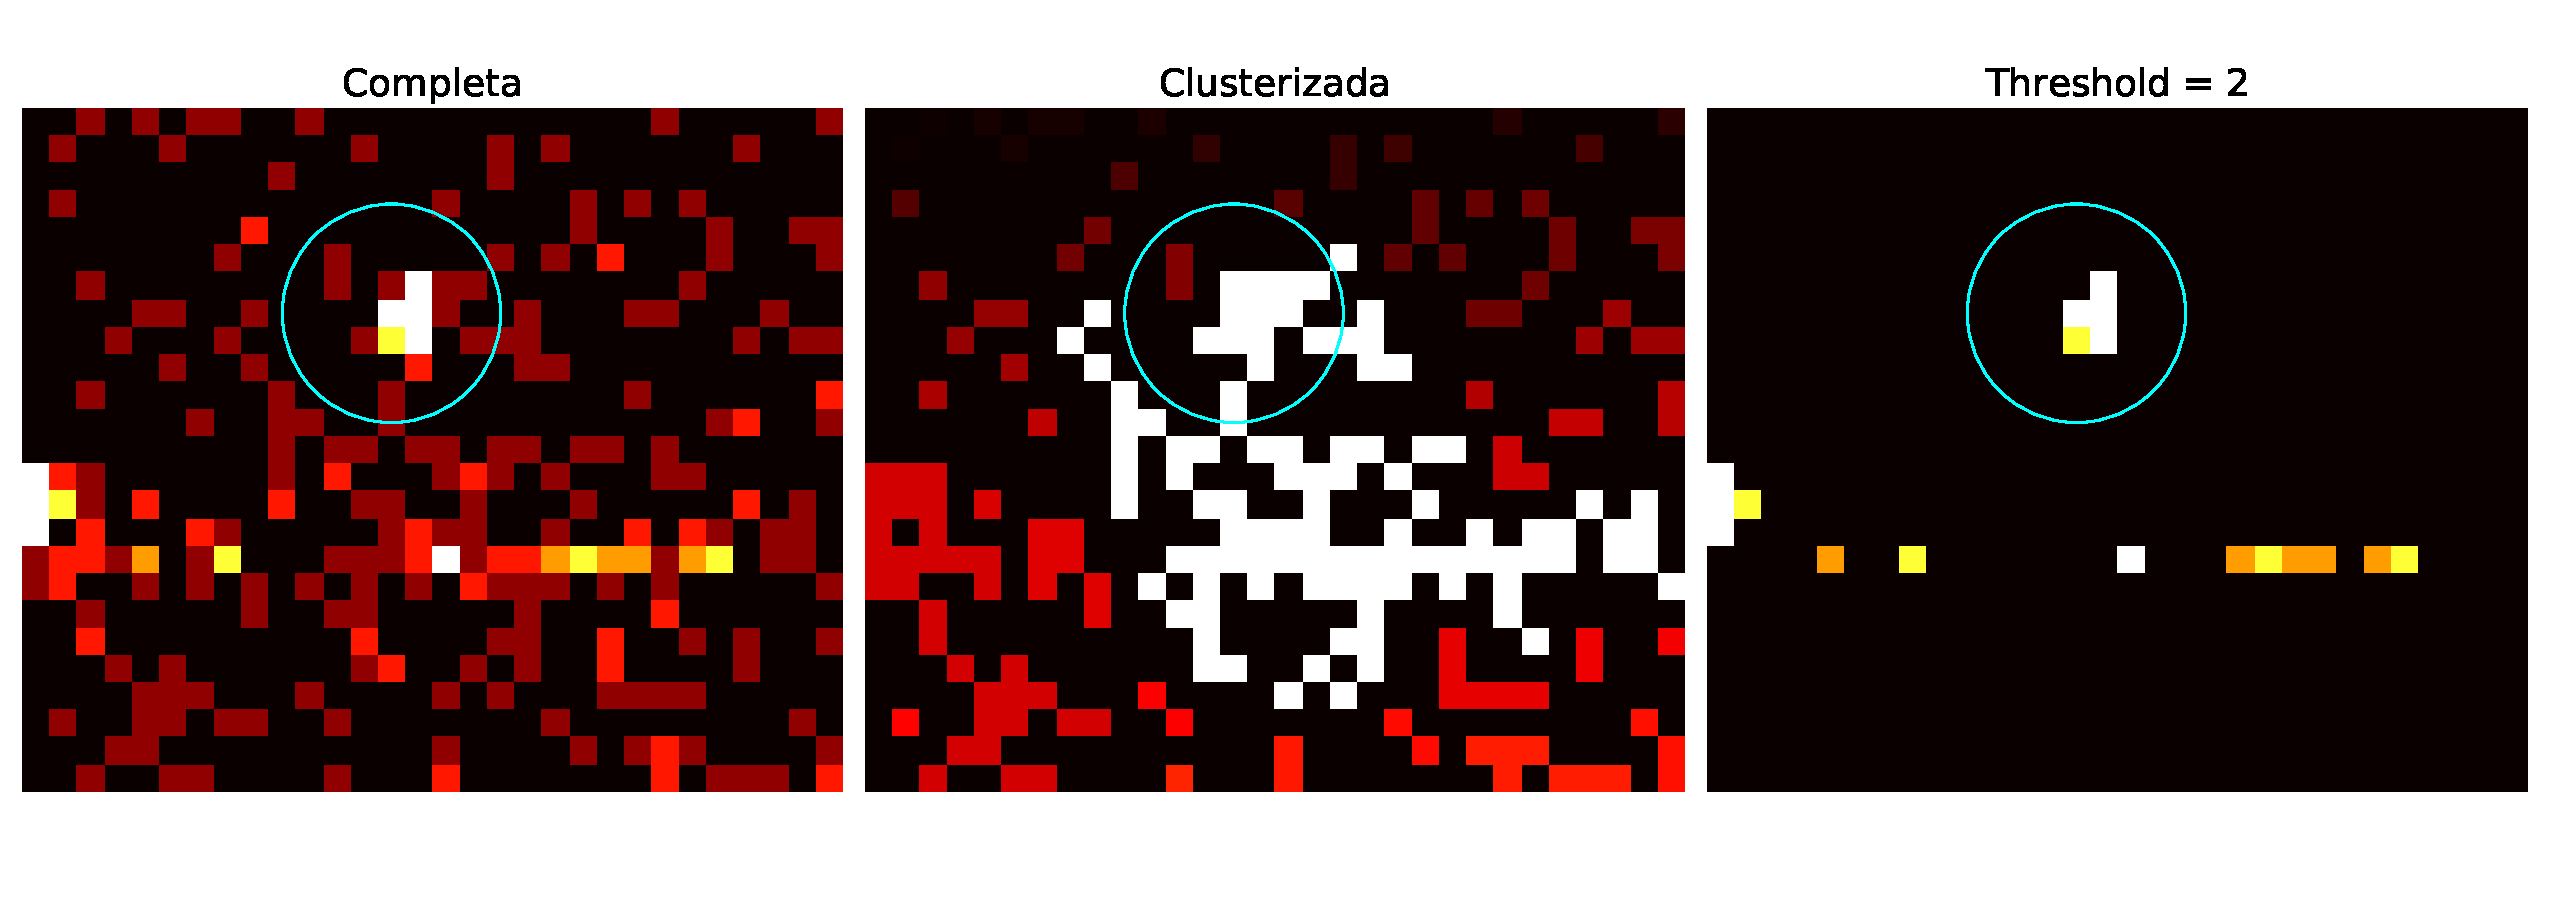
\includegraphics[scale=0.4]{Figs/despegoteo_clusters.pdf}
    \caption{\footnotesize{Ejemplo del caso de un de un evento cercano a los $180$ electrones de carga, que son los eventos de interés. En la imagen de la izquierda se ve la imagen completa, es decir, la medición sin alterar (ya convertida a unidades de carga). En la imagen del centro se ve en blanco y en un degrade muy tenue de rojos los diferentes clusters que el algoritmo logra reconocer. Lo importante de esta imagen es notar que el algoritmo reconoce como un unico cluster (blanco) a un número de píxeles muy grande debido justamente a que píxeles con una única carga generan la unión entre todos ellos. Por último, la imagen de la derecha contiene el cluster de interés una vez que los eventos de un electrón son desechados del análisis, haciendo que ahora sí se contabilice correctamente el evento de interés. Este es un evento de $174$ electrones de carga.}}
    \label{fig:ClusterPegoteado}
\end{figure}
De esta forma, se rehicieron los análisis de las imágenes con diferentes valores del corte de calidad, \verb|EPIX = 0.5|, \verb|EPIX = 1.5| y \verb|EPIX = 2.5| y se compararon los resultados obtenidos, tanto para el conteo total de eventos, como los valores finales del factor de Fano y la energía de creación electrón-hueco. Cabe aclarar que estos son resultados preliminares, debido a que la aplicación del umbral añade un sesgo extra al conteo de carga que posteriormente será corregido. Esto se hizo para tres de los cuatro cuadrantes del sensor, también llamados OHDU's, y se tuvo en cuenta la suma de los tres cuadrantes funcionales.\\
\indent En las figuras \ref{fig:EntradasVsEpix}, \ref{fig:EnergiadeCreacionVsEpix} y \ref{fig:FanoVsEpix}  puede verse la variación de estos parámetros dependiendo del valor de umbral usado. El gráfico más importante en este punto es el de la figura \ref{fig:EntradasVsEpix}, donde se observa un drástico aumento en la cantidad de entradas (eventos contabilizados) cuando se varía el \verb|EPIX|. Se graficaron en cada figura las modificaciones para tres de los cuatro cuadrantes del sensor y para la suma de los cuadrantes $1$, $3$ y $4$. El cuadrante $2$ no funciona correctamente y por eso sus datos no han sido utilizados.
\begin{figure}[h]
%Para hacer estas figs hay que ir a /home/igna/Escritorio/Tesis2021/Figs/pys_para_plots y correr plots_entries_fano_eh.py que usa los datos que están en /home/igna/Escritorio/Tesis2021/Figs/txts_para_plots y se llaman Entries_count.txt
    \centering
    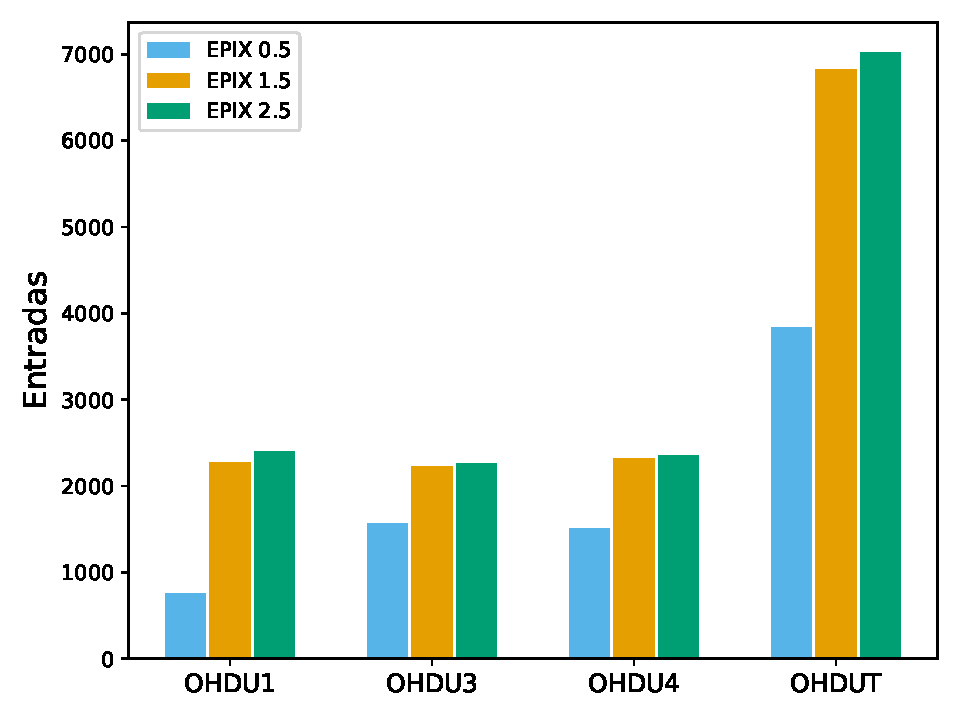
\includegraphics[scale=0.5]{Figs/Entradas_vs_Epix.pdf}
    \caption{\footnotesize{Gráfico de barras para las diferentes cantidad de entradas contabilizadas por el programa, tanto para valores diferentes de EPIX como para los diferentes cuadrantes del sensor. OHDUT hace referencia a la suma de las entradas del resto de los cuadrantes funcionales ($1$, $3$ y $4$). Se observa un aumento de más del doble en la cantidad en la cantidad de entradas para el primer cuadrante, y un aumento importante pero menos pronunciado para el resto de los cuadrantes.}}
    \label{fig:EntradasVsEpix}
\end{figure}
Se puede ver como los cuadrantes $1$, $3$ y $4$ tienen un cambio pronunciado en la cantidad de entradas al pasar de \verb|EPIX = 0.5| a \verb|EPIX = 1.5|, lo cual implica un aumento en la estadística, que era lo que se esperaba. En cambio, al pasar de \verb|EPIX = 1.5| a \verb|EPIX = 2.5| el aumento en el número de entradas es mucho menor. Particularmente, el primer cuadrante tiene un aumento muy importante en la cantidad de entradas en relación a los otros cuadrantes. Si bien el aumento sigue siendo pronunciado, para los cuadrantes $3$ y $4$ el aumento es menor. En la tabla \ref{tab:EntriesVsEpix} se presentan los valores precisos del cambio en el número de entradas para cada cuadrante para cada valor de \verb|EPIX|. El primer cuadrante pasa de tener $760$ entradas para \verb|EPIX = 0.5| a tener $2272$ para un \verb|EPIX = 1.5|, casi el triple, es un aumento de $\sim 198\%$. En cambio, los cuadrantes $3$ y $4$ pasan de tener $1571$ y $1503$ entradas a $2229$ y $2320$, un aumento muy similar y en torno al $\sim40\%$ y $\sim50\%$ respectivamente.
\begin{table}[h]
\centering
\begin{tabular*}{\textwidth}{c @{\extracolsep{\fill}}ccccc}%{@{}ccccc@{}}
\toprule
           & OHUD 1 & OHDU 3 & OHDU 4 & OHDU 1 + 3 + 4 \\ \hline\hline
EPIX = 0.5 & 760    & 1571   & 1503   & 3834           \\
EPIX = 1.5 & 2272   & 2229   & 2320   & 6821           \\
EPIX = 2.5 & 2399   & 2261   & 2356   & 7016           \\ \bottomrule
\end{tabular*}
\caption{\footnotesize{Diferentes valores para las entradas, para cada uno de los cuadrantes, para los diferentes valores de EPIX utilizados.}}
\label{tab:EntriesVsEpix}
\end{table}
Efectivamente se observa un aumento en el conteo de eventos que reconoce el programa al aumentar el valor del parámetro \verb|EPIX|. También se observa que el aumento más pronunciado es desde $0.5$ a $1.5$. El aumento promedio en el conteo de eventos es de alrededor del $100\%$.
\begin{figure}[h]
%Para hacer estas figs hay que ir a /home/igna/Escritorio/Tesis2021/Figs/pys_para_plots y correr plots_entries_fano_eh.py que usa los datos que están en /home/igna/Escritorio/Tesis2021/Figs/txts_para_plots y se llaman Entries_count.txt
    \centering
    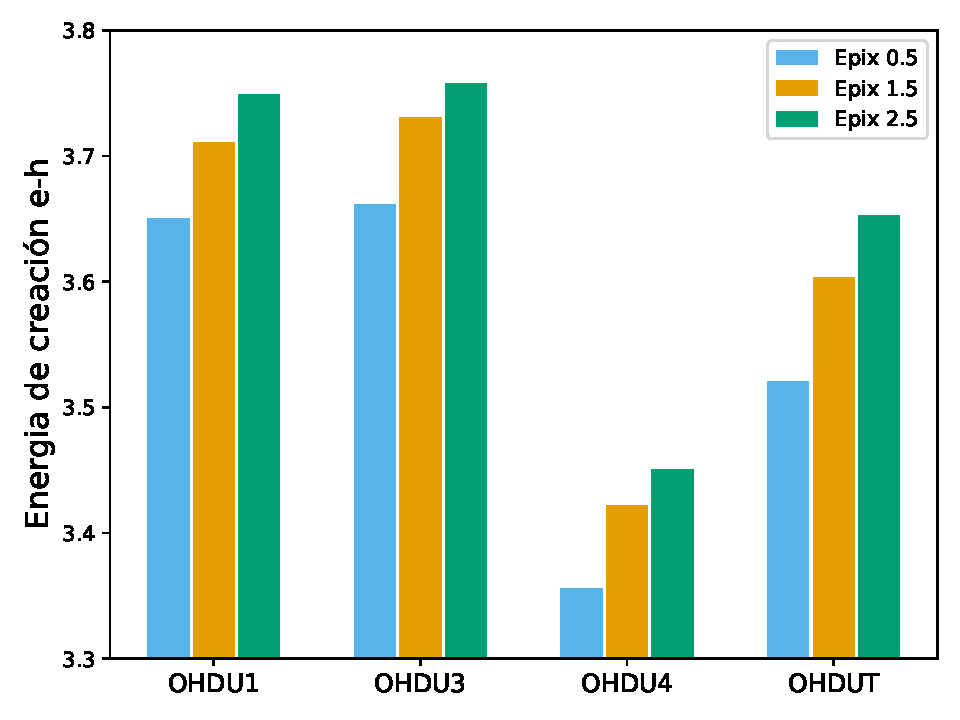
\includegraphics[scale=0.5]{Figs/EnergiaCreacion_vs_Epix.pdf}
    \caption{\footnotesize{Diferentes valores para la energía de creación electrón-hueco en función del EPIX y del cuadrante del sensor utilizado. OHDUT hace referencia a al promedio del resto de los cuadrantes funcionales ($1$, $3$ y $4$). Se observa que en todos los casos hay un aumento de la energía de creación electrón hueco cuando aumenta el EPIX.}}
    \label{fig:EnergiadeCreacionVsEpix}
\end{figure}
En cuanto al gráfico de la figura \ref{fig:EnergiadeCreacionVsEpix}, se ve como el valor preliminar para la energía de creación electrón hueco aumenta en todos los casos al aumentar el umbral \verb|EPIX|. Esto puede deberse al efecto que genera aplicar un umbral y disminuir la carga en los clusters contabilizados, que a su vez son más. Puede suceder que la cantidad de carga en los clusters sufra un corrimiento a la izquierda del valor medio real y por esto la energía de creación electrón-hueco aumente al aumentar el \verb|EPIX|: A un mismo valor de energía, una menor carga ionizada implica una mayor energía de creación electrón-hueco.
Finalmente, el caso más irregular corresponde al gráfico de la figura \ref{fig:FanoVsEpix}, donde cada cuadrante y para cada valor de \verb|EPIX| el factor de Fano dio valores diferentes y no puede definirse una tendencia a partir de estos resultados.
\begin{figure}[h]
%Para hacer estas figs hay que ir a /home/igna/Escritorio/Tesis2021/Figs/pys_para_plots y correr plots_entries_fano_eh.py que usa los datos que están en /home/igna/Escritorio/Tesis2021/Figs/txts_para_plots y se llaman Entries_count.txt
    \centering
    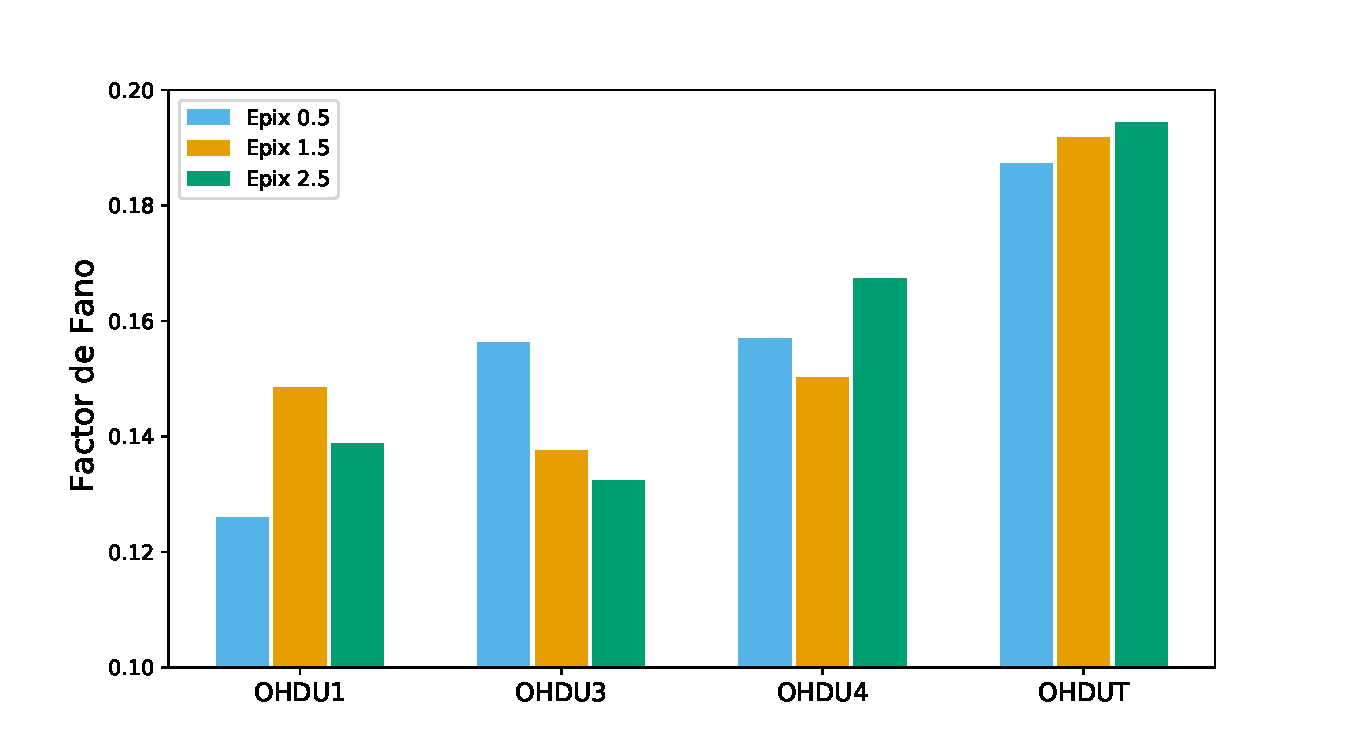
\includegraphics[scale=0.5]{Figs/Fano_vs_Epix.pdf}
    \caption{\footnotesize{Variación del factor de Fano en función del EPIX para diferentes cuadrantes del sensor. No se observa un patrón que se repita.}}
    \label{fig:FanoVsEpix}
\end{figure}
Entonces, del análisis preliminar modificando el umbral conteo de carga por píxel se puede observar el aumento deseado en la estadística para los eventos de interés de este trabajo. Como se observa que el mayor aumento en la estadística se da para \verb|EPIX = 1.5|, ese es el valor de umbral con el que se realizan los subsiguientes análisis. No está de más recordar que ese valor de umbral implica desechar los píxeles que tengan menos de $2$ electrones de carga.\\
\indent Habiendo tomado este rumbo, es necesario poder remover el sesgo producido por la eliminación de carga en los eventos medidos. Si bien definir un umbral genera un aumento en la estadística, también genera un corrimiento hacia la izquierda en los picos de interés en los espectros que debe ser corregido. Más aún, es necesario remover además el exceso de carga que tengan los clusters de interés debido a corrientes oscuras o eventos indeseados que generen un corrimiento a la derecha de los picos en los espectros. En adelante, la idea es intentar comprender el ruido de fondo en las imágenes y con ello poder corregir los valores de carga de los clusters, una vez aplicado el umbral y así mejorar la incerteza de los resultados.

%%%%%%%%%%%%%%%%%%%%%%%%%%%%%%%%%%%%%%%%%%%%%%%%%%%%%%%%%%%%%%%%%%
\section{Caracterización de las imágenes}
\noindent Todo el análisis cuantitativo anteriormente descripto se realizó sin la necesidad de inspeccionar visualmente las imágenes de las cuales se extraen los datos. Simplemente se aplicaron diferentes umbrales de prueba y se contabilizó el aumento en la estadística. Sin embargo, ver las imágenes y rápidamente poder reconocer patrones, como exceso de eventos en una misma región para diferentes imágenes o cualquier característica que visualmente sea reconocible pero que al analizar los datos de forma automatizada pueda quedar ofuscada, es un factor importante a la hora del estudio de los datos. Dado que la cantidad de imágenes utilizadas en este trabajo es superior a las $900$, claramente observar una por una es una tarea monumental y sin sentido. Por esta razón fue necesario buscar maneras de poder extraer información contenida en todas las imágenes, de forma práctica y realizable, como por ejemplo, generar una imagen \textit{promedio} de todas las imágenes. Con este fin, se hizo un análisis visual, cualitativo y cuantitativo de las imágenes para comprender mejor los datos, explorar las características del sensor y de cada uno de sos cuadrantes y poder reconocer posibles deficiencias o cualquier tipo particularidad relevante.\\
\indent Uno de los primeros factores a caracterizar tiene que ver con la carga de los píxeles que no es debida ni a eventos de ionización ni a eventos de interés. Estos pueden ser producto de corrientes oscuras (electrones que sufren excitaciones espontáneas debido a fluctuaciones térmicas del sensor), rebotes de un haz de baja energía en la cámara donde se encuentra el sensor y producen eventos que no son de interés en un determinado píxel, etc. No es sencillo y no existe una única manera de estimar el fondo en un sensor, por lo que en este trabajo se ensayaron deferentes maneras de encarar este análisis. \\
\indent Lo primero que se hizo en este trabajo fue buscar la manera de explorar solamente los píxeles que tuvieran una única carga. Asumiendo que en la gran mayoría de los casos, los píxeles con una única carga que se encuentran aislados de otros píxeles o de clusters de interés, son eventos que forman parte del fondo del sensor, es natural empezar el análisis con estos. Una forma de caracterizar esto es tomar las imágenes y extraer todos los píxeles donde la carga sea mayor que un electrón. De este modo, se obtienen imágenes donde solo hay eventos de un electrón y todo lo demás son píxeles vacíos. En la figura \ref{fig:ImagenFitsOriginal} se puede ver una típica imagen tomada con el sensor, para el primer cuadrante, en la que claramente pueden observarse algunos eventos muy brillantes y un intenso fondo. En la imagen \ref{fig:ImagenFits1e} en cambio puede verse la imagen resultante de extraer todos los píxeles cuya carga sea mayor a $1$ electrón.
\begin{figure}[h]
%Para hacer estas figs hay que ir a /home/igna/Escritorio/Tesis2021/Figs/pys_para_plots y correr imagenes_fits_original_y_filtrada.py
    \centering
    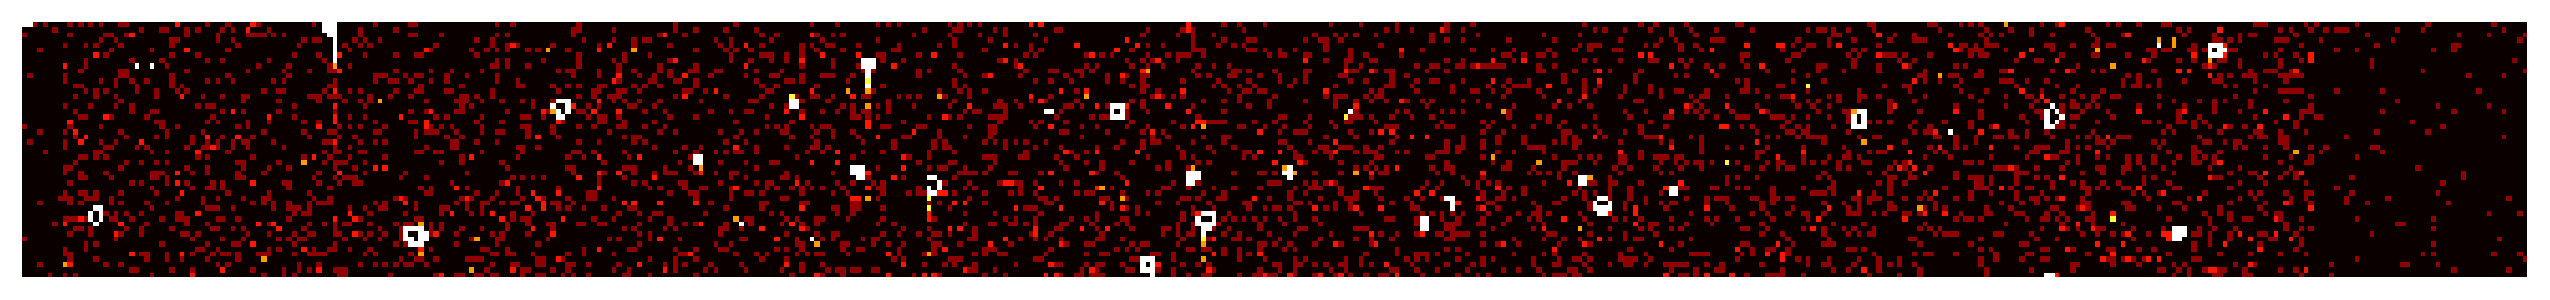
\includegraphics[scale=0.4]{Figs/imagen_fits_original.pdf}
    \caption{\footnotesize{Ejemplo de imagen tomada con el sensor, en el primer cuadrante.}}
    \label{fig:ImagenFitsOriginal}
\end{figure}

\begin{figure}[h]
%Para hacer estas figs hay que ir a /home/igna/Escritorio/Tesis2021/Figs/pys_para_plots y correr imagenes_fits_original_y_filtrada.py
    \centering
    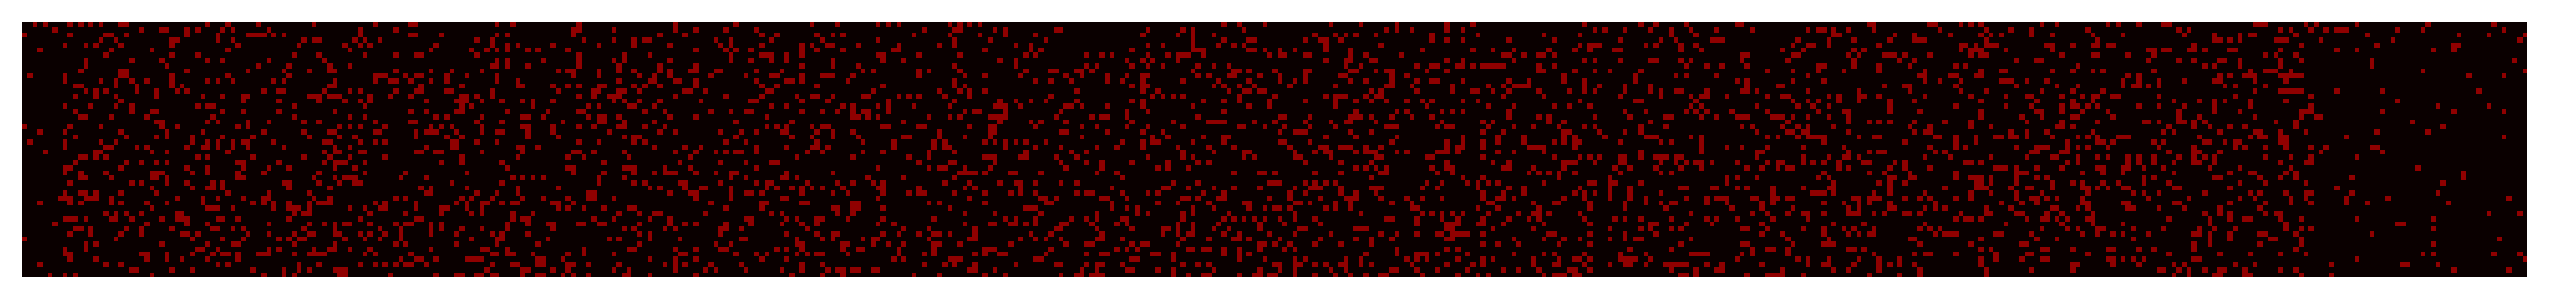
\includegraphics[scale=0.4]{Figs/imagen_fits_1_e.pdf}
    \caption{\footnotesize{Imagen resultante luego de ser extraídos los píxeles con carga mayor a $1$ electrón.}}
    \label{fig:ImagenFits1e}
\end{figure}
Una vez que se extraen los píxeles de carga mayor a $1$, se promedian todas las imágenes resultantes y se obtiene una una única imagen que condensa la información de todas las anteriores. En este contexto, promediar las imágenes implica tomar el objeto matricial de valores ($0$ y $1$ en este caso) de carga en cada píxel (cada elemento fila y columna de la matriz) para cada imagen, y realizar la suma convencional de matrices para las $\sim 950$ imágenes. Finalmente dividir cada elemento de la matriz por la cantidad total de imágenes. De esta forma se puede ver si existen píxeles con mayor o menor tendencia a contener este tipo de eventos.\\
\indent En la figura \ref{fig:Eventos1e} se tiene una imagen por cada cuadrante del sensor, promediados en las $925$ imágenes tomadas, donde los píxeles más brillantes son los que tienen mayor promedio de eventos, es decir, en el total de las imágenes esos píxeles son los que más veces tuvieron un electrón de carga. Esto también puede interpretarse como una imagen de la probabilidad por píxel de que haya un único electrón: Píxeles más brillantes son píxeles más propensos a tener carga y los píxeles más oscuros los menos propensos.\\
\indent De la figura \ref{fig:Eventos1e} pueden destacarse algunas características:
\begin{itemize}
    \item La carga prácticamente nula (en promedio) en las regiones del pre-scan (región izquierda de $8$ columnas de píxeles de extensión) y del over-scan (región derecha de 50 columnas de píxeles de extensión), lo cual es totalmente esperable, para todos los cuadrantes menos el segundo;
    \item El primer cuadrante es en promedio más brillante que el resto, y se observa un ligero gradiente de intensidad entre las filas inferiores y superiores. Esto se repite, pero en menor medida en los demás cuadrantes pero no necesariamente se observa a simple vista;
    \item El segundo cuadrante (OHDU 2) capta en promedio muy poca carga. Este cuadrante del sensor es defectuoso;
    \item En los cuadrantes $3$ y $4$ se pueden ver columnas enteras de píxeles oscurecidas, que captaron muchísima menos carga que podrían deberse a defectos del sensor;
    \item En todos los cuadrantes (menos el segundo), se observa un único píxel (posición $x = 2$, $y = 0$) donde el promedio de carga es mucho mayor al resto. Además, la primera columna de píxeles luego del pre-scan también tiene tendencia a captar más carga que el resto;
    \item Todos los cuadrantes tienen tendencia a tener \textit{hot píxels} en el interior de la región activa, esto es píxeles aislados que tienden a tener más carga que otros, además pueden verse lineas verticales de \textit{hot píxeles} que no pueden explicarse completamente.
\end{itemize}
\begin{figure}[h]
%Para reproducir esta figura hay que ir al directorio /home/igna/Escritorio/Tesis2021/Figs/pys_para_plots y correr Skipper_cuadrantes_plot.py
    \centering
    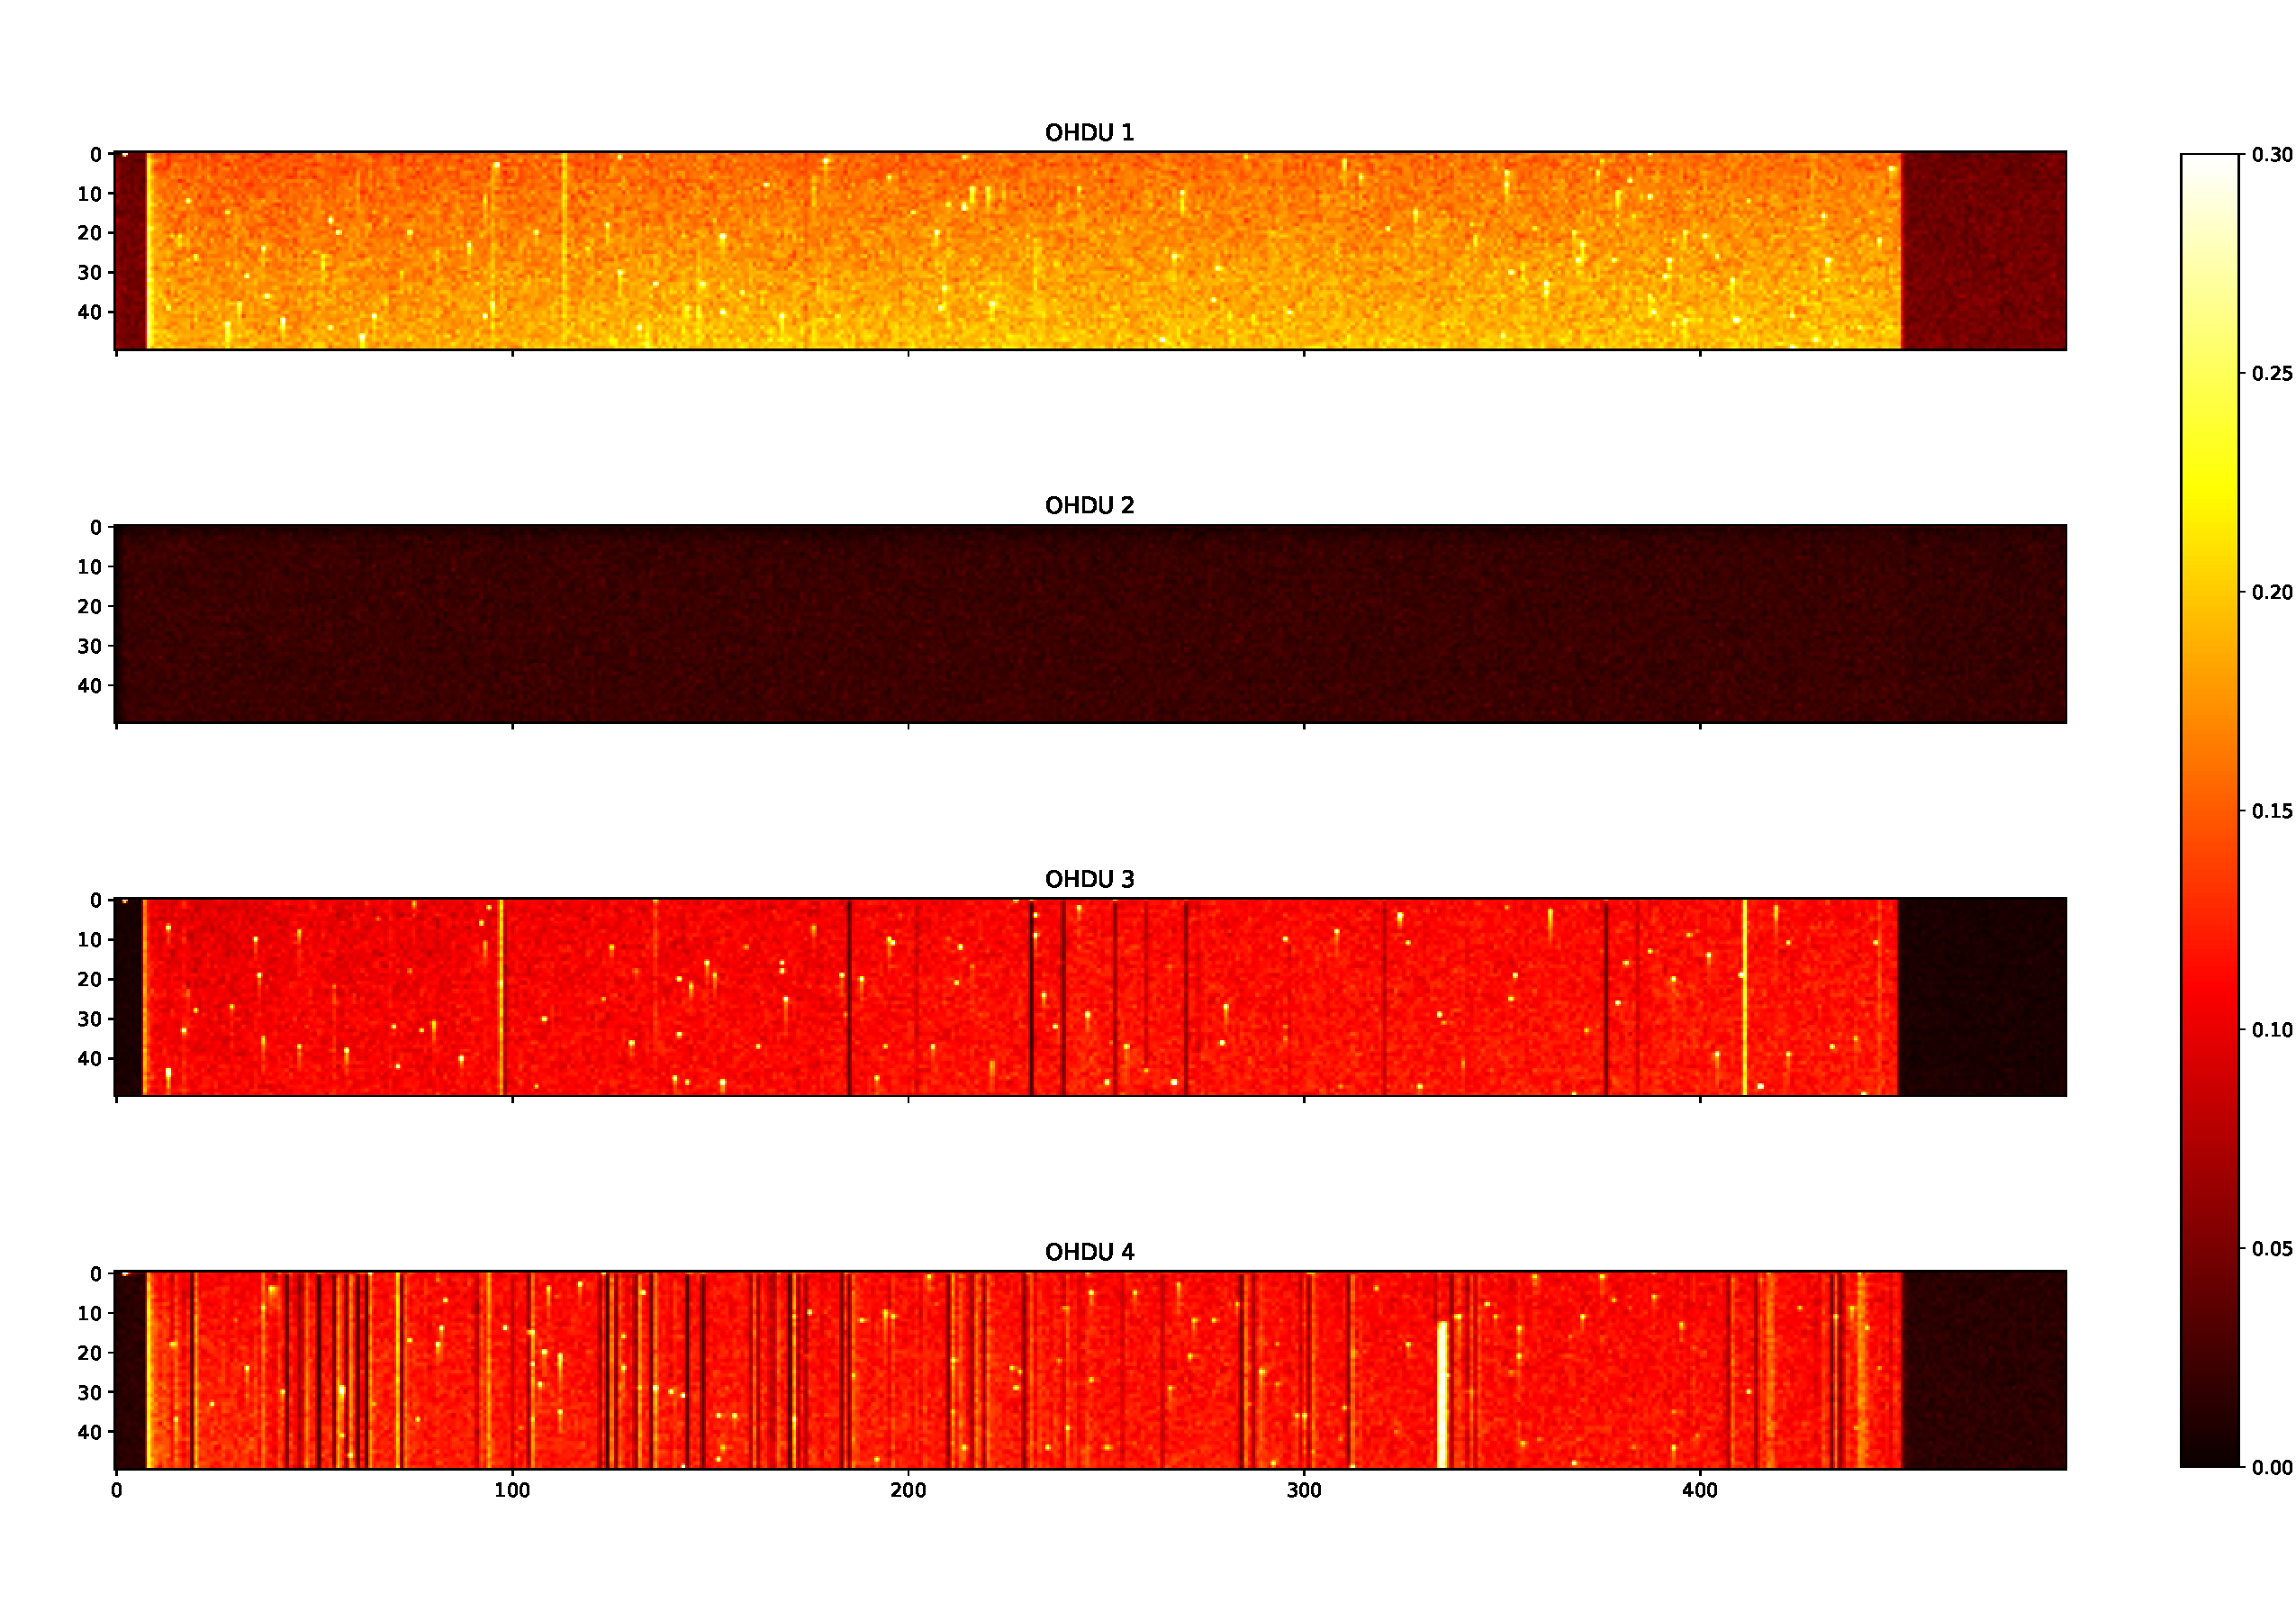
\includegraphics[scale=0.4]{Figs/1ePromedio.pdf}
    \caption{\footnotesize{Imágenes promedio para los $4$ cuadrantes del sensor. Puede verse en la escala de la derecha que los valores más altos que se obtienen rondan el $0.3$, lo cual, interpretado como una probabilidad es un $30\,\%$ de probabilidad de que en ese píxel se encuentre un evento de un electrón. En general se ve que los promedios pueden estar entre $0.1$ y $0.2$ aproximadamente. Es decir, para los cuadrantes funcionales del sensor, cada pixel tiene una probabilidad de tener un único evento que ronda entre el $10\%$ y el $20\%$.}}
    \label{fig:Eventos1e}
\end{figure}
Respecto al gradiente de intensidades que se observa entre filas superiores e inferiores, implicaría una mayor incidencia de eventos de un electrón, en promedio, en los píxeles de las filas inferiores respecto de las filas superiores. Esto puede observarse en los gráficos de figura \ref{fig:GradienteProb}, donde se ve el aumento en \textit{la probabilidad} media por fila de que haya un evento de un electrón, a medida que el número de la fila aumenta. El gráfico de arriba a la izquierda corresponde al primer cuadrante del sensor, este es el cuadrante donde más evidente se hace este gradiente, además de ser muy lineal. La probabilidad promedio para la fila $0$ del sensor es $\sim 14.5\,\%$ y crece linealmente hasta $\sim 18\,\%$ para la fila $50$. En el gráfico de arriba a la derecha, que corresponde al segundo cuadrante, también se observa un cambio, pero solo entre las primeras 10 filas del sensor, luego la variación de la probabilidad por fila es muy pequeña y parece aproximadamente constante. Además puede verse que los valores son un orden de magnitud menor a los del primer cuadrante. Para los gráficos de abajo a la izquierda y abajo a la derecha, que corresponden a los cuadrantes $3$ y $4$ del sensor respectivamente, se observan también variaciones entre las primeras filas del sensor y las últimas que parecerían tener una tendencia lineal, sin embargo, en comparación a la variación del primer cuadrante, esta es mucho menor. Por esto es difícil verlo a simple vista: la variación para el primer cuadrante es de aproximadamente del $24\,\%$ mientras que la variación de los cuadrantes $3$ y $4$ es aproximadamente del $10\,\%$.\\
\indent Esto se debe a que, dado que la medición de carga del sensor es secuencial, las filas superiores son las primeras a las que se les mide la carga, generando que las filas inferiores permanezcan más tiempo expuestas a fuentes de fondo. De todas maneras esta diferencia de tiempo en la lectura de las diferentes filas del sensor es muy pequeña, haciendo que estas diferencias entre filas sea pequeña, aunque apreciable en algunos casos.\\
\begin{figure}[h]
%Para modificar este plot hay que ir a /home/igna/Escritorio/Tesis2021/Figs/pys_para_plots y correr gradiente_filas_sensor.py Los datos los saca de /home/igna/Escritorio/Tesis2021/Figs/txts_para_plots y del archivo OHDU1/2/3/4_gradiente_filas_sensor.tx
    \centering
    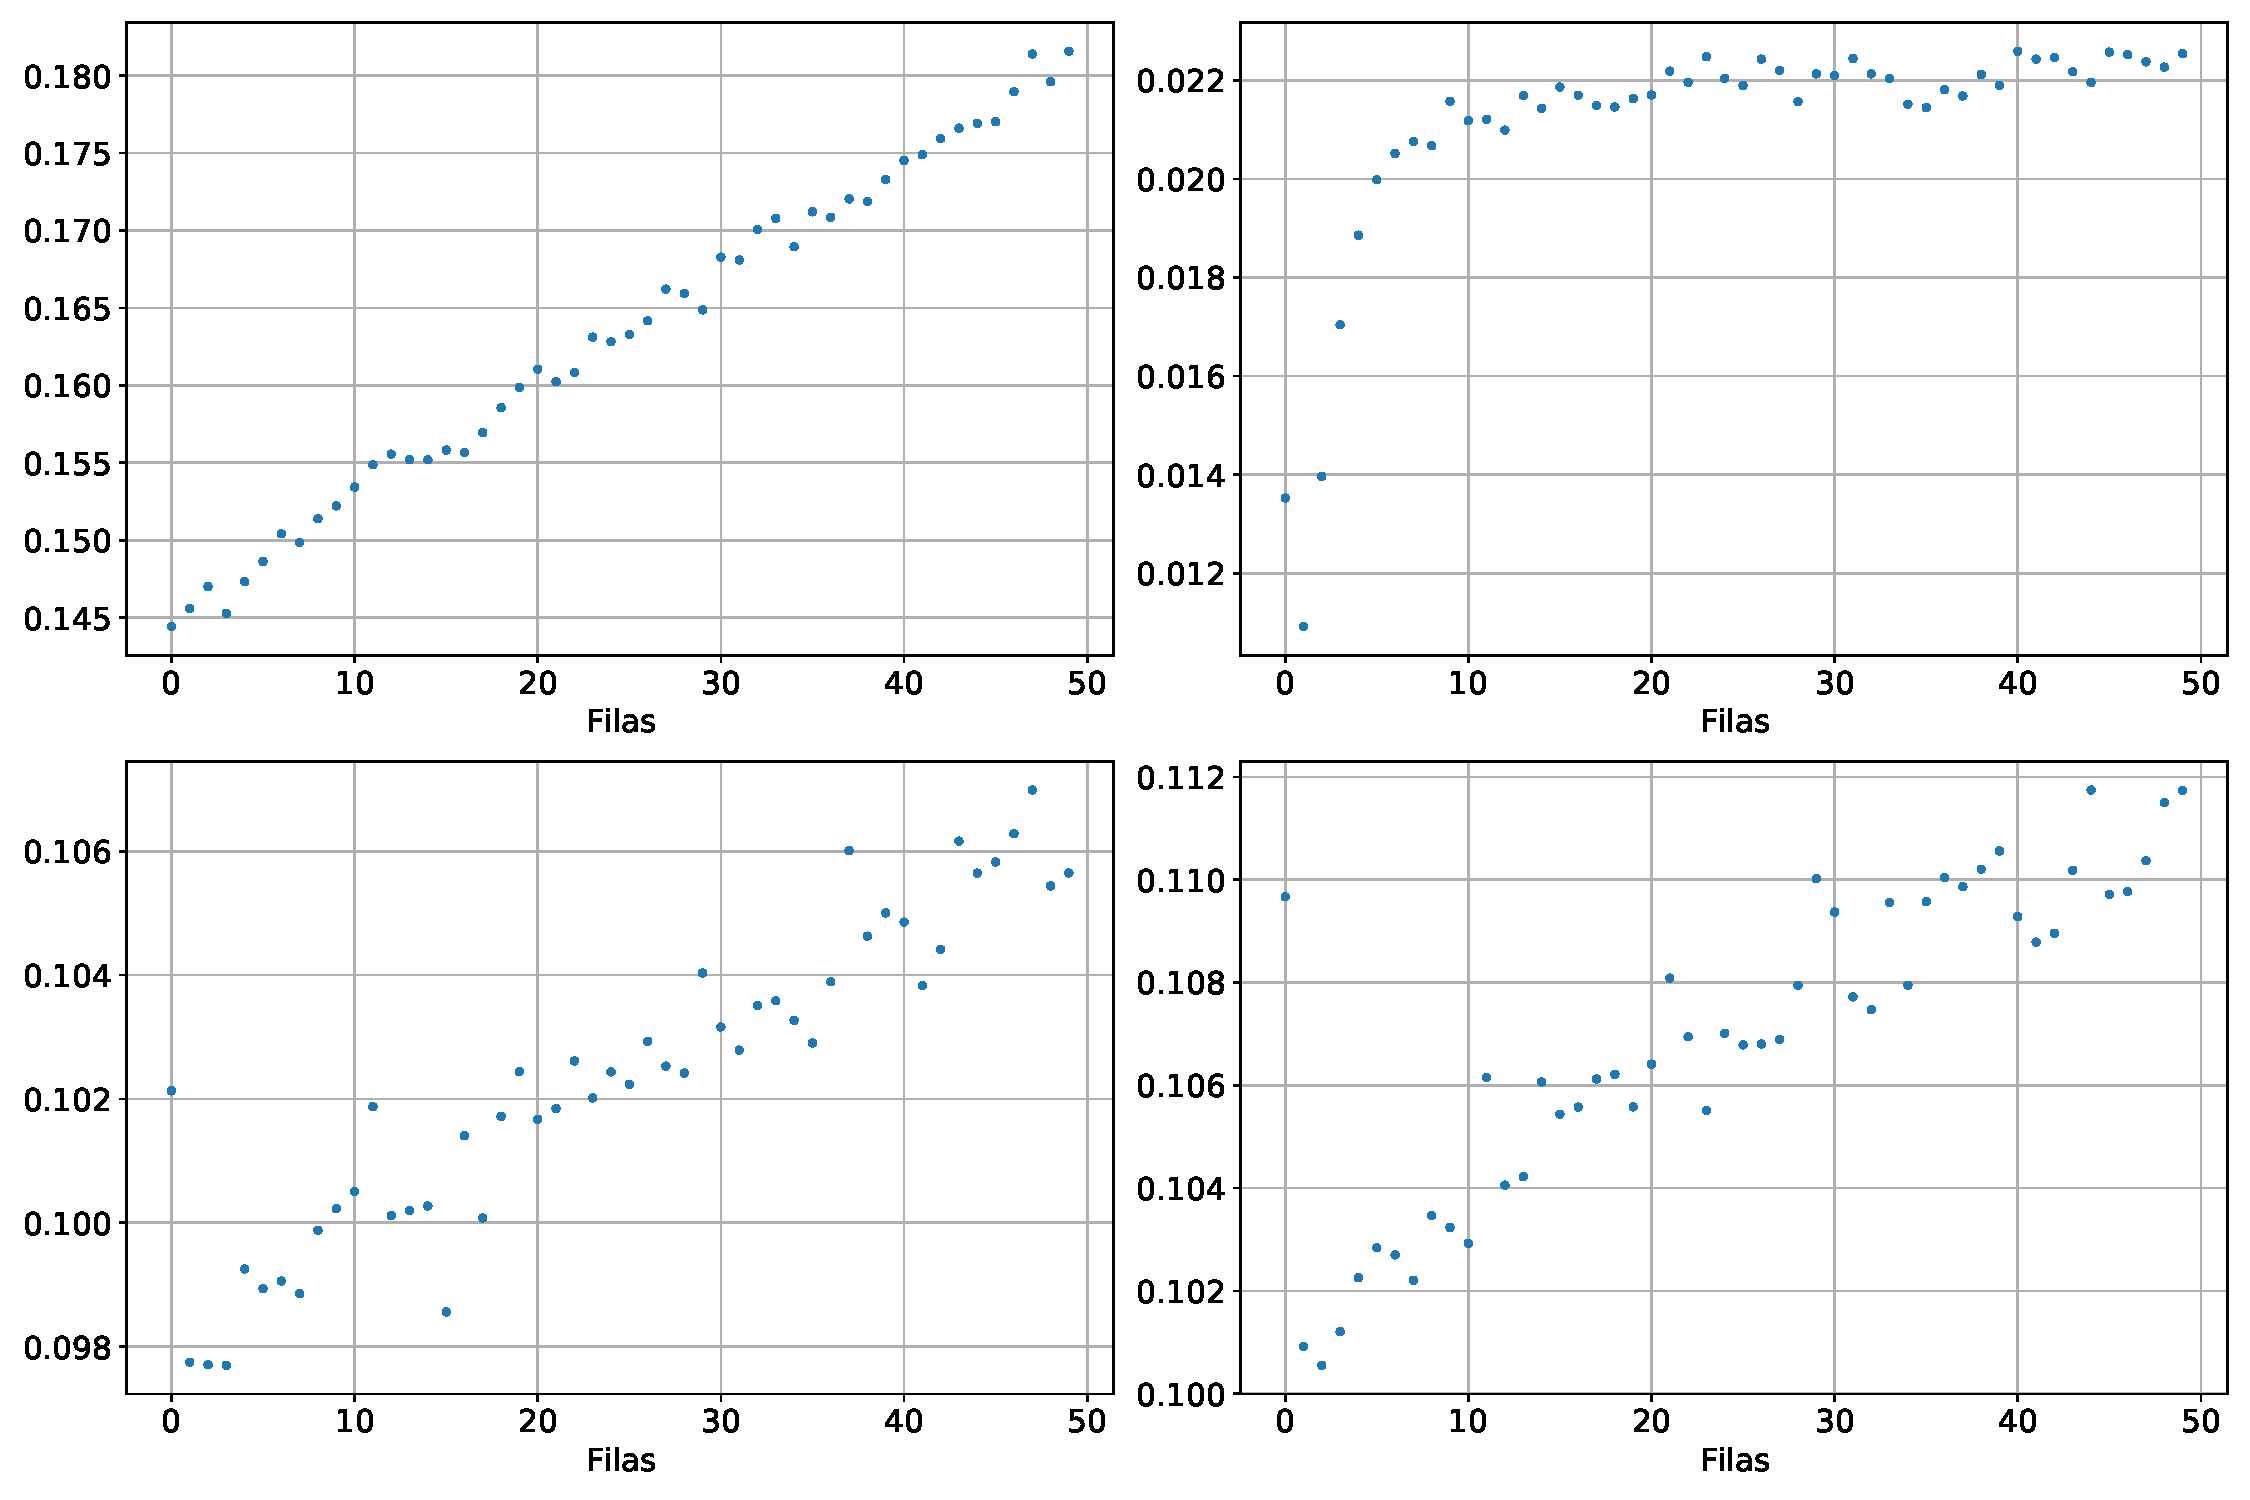
\includegraphics[scale=0.45]{Figs/Gradiente_en_filas_sensor.pdf}
    \caption{\footnotesize{Variación de la \textit{probabilidad} promedio por filas del sensor de tener un evento de $1$ electrón, para los diferentes cuadrantes. Se ven aumentos lineales de la probabilidad para los casos de los cuadrantes $1$, $3$ y $4$ y un aumento más pronunciado en relación a los demás para el primer cuadrante.}}
    \label{fig:GradienteProb}
\end{figure}
\indent Todos los análisis subsiguientes fueron realizados principalmente con el primer cuadrante del sensor, dado que es el cuadrante que funciona mejor.\\
\indent Teniendo entonces una imagen del promedio de la cantidad de eventos de un electrón por píxel, en la búsqueda por caracterizar el fondo del sensor, lo que se hizo posteriormente fue promediar todos los elementos de esta, de forma de obtener un promedio total y poder interpretarlo como una \textit{probabilidad} general de que en un píxel haya un evento de un electrón. Entonces, para el primer cuadrante y considerando solo la región activa del sensor, se obtuvo una probabilidad $p = 0.176 \pm 0.021$, es decir, que con esta primera manera de caracterizar el fondo, hay aproximadamente un $17\,\%$ de probabilidad de que un dado píxel de la región activa del sensor tenga un electrón.\\
\indent Sin embargo, esta es una forma muy rudimentaria para intentar caracterizar el ruido del sensor, además de que no es del todo correcta. Con este camino se asume que todos los eventos de un electrón vienen del fondo, lo cual claramente no es correcto, de forma que la probabilidad de tener un evento de un electrón en un dado píxel, calculada de esta manera, está sobrestimada. Un camino más sofisticado para estimar el ruido en el sensor es explotando el hecho de que los eventos medidos en él siguen una distribución Poissoniana: Si se supone que todo píxel tiene igual probabilidad de tener una carga debido a fondo, que dicha probabilidad es pequeña para mediciones de corto tiempo y que el número de píxeles es muy grande ($24650$ píxeles por cuadrante), entonces es esperable que la distribución que modela estos eventos sea una Poissoniana. De esta forma, si se pudiera calcular la esperanza $\mu$ de la distribución, podría saberse la probabilidad de que en un determinado píxel se encuentre un evento de un electrón o, en general, la cantidad de electrones que se deseé.\\

\section{Estimación de la esperanza de la distribución}
\noindent Si se considera una distribución Poissoniana para la variable aleatoria \textit{número de electrones de fondo por píxel}, se puede tomar el caso $p = P(k = 1 | \mu) = 0.176 \pm 0.021$, que es la probabilidad que se obtuvo previamente. De forma iterativa puede hallarse el valor de $\mu$ que satisface la expresión anterior y resulta:
\begin{equation*}
    \mu = 0.2194 \pm 0.0001
\end{equation*}
Si bien esta forma de cuantificar el fondo es un poco más general, dado que ahora pueden contemplarse casos más raros, como que un píxel tenga más de una carga producto de corrientes oscuras u otros factores, este método sigue teniendo el problema de la sobrestimación de la probabilidad por píxel, al seguir asumiendo que todo píxel con un electrón proviene del fondo. Por otro lado, esta forma también presenta el inconveniente que para calcular la probabilidad hubo que hacer dos promedios, primero un promedio sobre todas las imágenes y luego un promedio sobre todos los píxeles.\\
\indent Siguiendo sobre el mismo camino, todavía bajo la hipótesis de que todo evento de un electrón es debido a fondo, pero evitando el cálculo de los promedios, hay una forma de calcular la esperanza de la distribución y es notando lo siguiente: Si se toman las probabilidades de que haya una sola carga y ninguna carga por píxel, es decir, se toman
\begin{equation*}
    p_{0} \equiv P(k = 0 | \mu),
    \quad
    \quad
    p_{1} \equiv P(k = 1 | \mu)
\end{equation*}
y se mira la relación entre ambas, se tiene
\begin{equation*}
    \frac{p_{1}}{p_{0}} = \frac{\mu\,e^{-\mu}}{e^{-\mu}} = \mu
\end{equation*}
y se ve que puede hallarse directamente el valor de la esperanza de la distribución. Entonces, tomando la región activa de una imagen original (sin separar los eventos de $1$ o más electrones), como la de la figura \ref{fig:ImagenFitsOriginal}, contando la cantidad de píxeles vacíos, la cantidad de píxeles con $1$ electrón y calculando la relación entre ambas, para todas las imágenes, se puede obtener directamente la esperanza $\mu$ de la distribución. De esto se obtuvo que el valor de la esperanza es:
\begin{equation*}
    \mu = 0.2245 \pm 0.0001
\end{equation*}
Los resultados de ambos métodos son parecidos, aunque presentan diferencias significativas ya que no se solapan sus errores. Si bien esta segunda forma para calcular la esperanza $\mu$ parece un poco más elegante y correcta, el problema sigue estando en los datos que se utilizan. El valor seguirá estando sobrestimando respecto del valor real, en tanto se considere a todo píxel con un único electrón como fondo.\\
\indent No hay que perder de vista que el objetivo de calcular la esperanza de la distribución es poder utilizarla para estimar cuánta carga extra hay sobre los clusters debida a fondo y cuánta carga no espuria fue removida debido al umbral aplicado. Conociendo la esperanza de la distribución del ruido y la cantidad de píxeles que ocupa un cluster, puede calcularse la cantidad esperada de carga extra debido a fondo que se halla en cada cluster. Teniendo estos valores, puede corregirse el valor de la carga y con eso hacer mejores estimaciones del factor de Fano y la energía de creación electrón-hueco.\\
\indent Pero también, para poder generar una corrección en el conteo de cargas por cluster y que esté lo menos sesgada posible, hay que tener en cuenta las posibles formas en las que un cluster podría tener más o menos carga:
\begin{itemize}
    \item Que sobre la superficie de los clusters hayan eventos de más, debido a corrientes oscuras o cualquier forma de fondo del sensor;
    \item dado que en este análisis se está aplicando un umbral que elimina eventos de $2$ o menos electrones, podría suceder que a un cluster se le quiten eventos reales que se encuentran en sus bordes.
\end{itemize}
Con lo cual no solo es necesario corregir la carga por exceso en los clusters, sino también por defecto. Por ello, la esperanza que se obtuvo de calcular la relación entre eventos de $1$ electrón y píxeles vacíos contiene tanto información de eventos espúrios como información de eventos genuinos. Pero lo que se persigue es poder identificar los eventos espurios y los genuinos por separado. En ese sentido puede decirse que 
\begin{equation*}
    \mu_{T} = \mu_{bkg} + \mu_{g}
\end{equation*}
donde $\mu_{bkg}$ es la esperanza de la distribución de la variable aleatoria \textit{cantidad de eventos espurios por píxel}, mientras que $\mu_{g}$ es la esperanza de la variable aleatoria \textit{cantidad de eventos genuinos por píxel}. Hay que lograr separar ambos efectos para poder aplicar las correcciones correctamente. Queda claro que hasta el momento solo se calculó $\mu_{T}$, sin poder discriminar ambas contribuciones. La forma en la que se llevó a cabo la separación entre ellas se detalla a continuación.

\subsection{Análisis de los bordes de los clusters}
\noindent Para poder separar ambas contribuciones al calcular el $\mu_{T}$ de la distribución, la idea fue analizar los bordes de los clusters, donde ahora por clusters se entiende todo píxel individual de $2$ o más electrones de carga, o conjunto de píxeles donde cada uno tenga como mínimo $2$ electrones de carga. Es decir, se toma una imagen que tiene eventos de $2$ o más electrones, y los demás eventos se hacen $0$, como se ve en la figura \ref{fig:ImagenFits2omasElectrones}.
\begin{figure}[h]
%Para modificar este plot hay que ir a /home/igna/Escritorio/Tesis2021/Figs/pys_para_plots y correr imagen_fit_2_o_mas_e.py
    \centering
    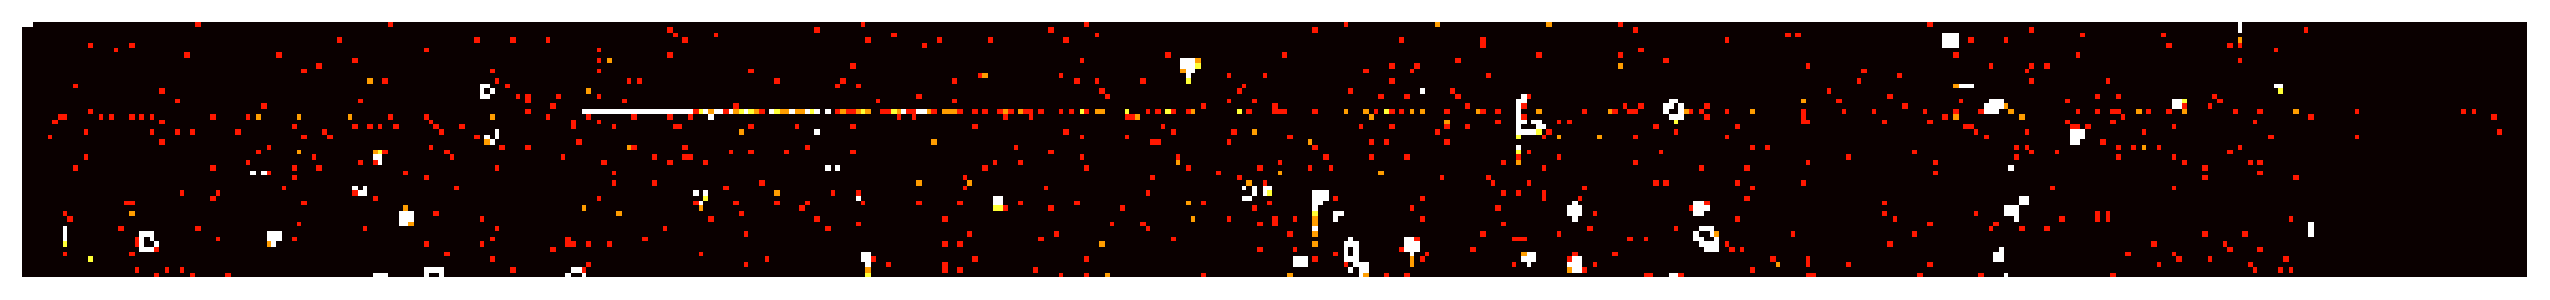
\includegraphics[scale=0.4]{Figs/imagen_fits_2_o_mas.pdf}
    \caption{\footnotesize{Imagen de ejemplo en la que solo hay píxeles que tenga más de $2$ electrones.}}
    \label{fig:ImagenFits2omasElectrones}
\end{figure}
Usando como referencia los clusters de esta imagen, se genera una máscara sobre de los bordes de estos, es decir, los píxeles inmediatamente contiguos a los píxeles con carga. Como la idea es corregir la carga en los clusters, tiene sentido mirar en el entorno de estos y no en todo el sensor.\\
\indent El procedimiento consiste en tomar los clusters y hacer una máscara de su contorno, con lo cual la máscara es el conjunto de píxeles que rodea al cluster, sin incluir los píxeles cargados. Luego, superponiendo la máscara sobre la imagen original (ahora con todos los eventos), se cuenta cuántos eventos cayeron dentro de la máscara. 
\begin{figure}[h]
%Para modificar este plot hay que ir a /home/igna/Escritorio/Tesis2021/Figs/pys_para_plots y correr imagen_bordes2.py
    \centering
    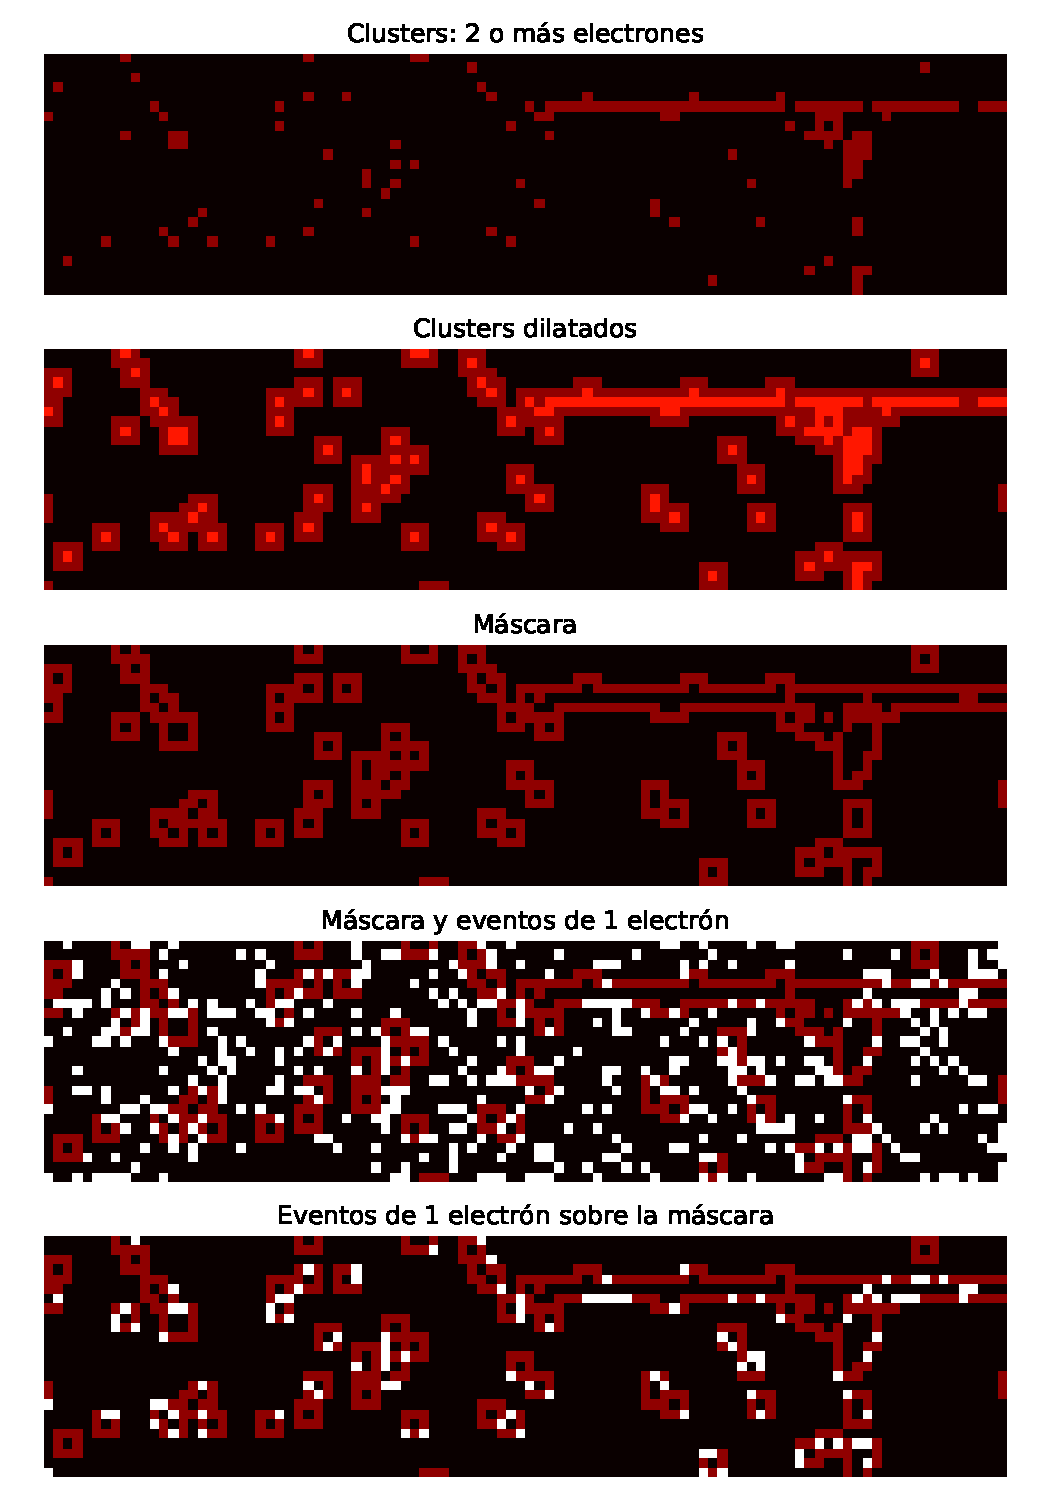
\includegraphics[scale=0.7]{Figs/analisis_bordes.pdf}
    \caption{\footnotesize{Diferentes partes del proceso de análisis de los bordes de los clusters para una imagen de ejemplo. En cada figura se ve una porción de $25 \times 100$ píxeles de área. En la primera imagen (de arriba a abajo) se tienen los clusters de $2$ o más electrones. En la segunda imagen se representa la dilatación de los clusters aumentando en $1$ píxel en todas las direcciones. En la tercera imagen se ve la diferencia entre las dos primeras imágenes y se la define como la máscara a utilizar. En la cuarta se ve la máscara y superpuestos todos los eventos de $1$ electrón de esa porción del sensor. Finalmente, en la quinta se ven solo los eventos de $1$ electrón que cayeron encima de los píxeles de máscara. Son estos eventos los que son se cuentan en todas las imágenes, junto con los píxeles vacíos de la máscara para calcular el $\mu_{T}$.}}
    \label{fig:AnalisisBordes}
\end{figure}
Nuevamente, haciendo la relación entre eventos de un electrón y píxeles vacíos, se calcula el $\mu_{T}$. En la figura \ref{fig:AnalisisBordes} puede verse gráficamente cada uno de los pasos que se lleva a cabo para contabilizar los eventos de $1$ electrón que caen sobre la máscara. Se estima que en el borde inmediato a los clusters existe contribución de ambos efectos: eventos espurios y eventos genuinos.\\
\indent Por otro lado, para calcular la contribución de los eventos espurios, se hace el mismo procedimiento pero expandiendo los clusters en dos píxeles en todas las direcciones, y quedándose únicamente con el segundo borde, donde claramente no puede haber contribución de eventos genuinos de un cluster. Este proceso puede verse en la imagen \ref{fig:AnalisisBordesx2}. Nuevamente, de la relación entre los eventos de $1$ electrón y los píxeles vacíos, se obtiene $\mu_{bkg}$ y con este, puede despejarse el valor $\mu_{g}$.\\

\begin{figure}[h]
%Para modificar este plot hay que ir a /home/igna/Escritorio/Tesis2021/Figs/pys_para_plots y correr imagen_bordesx2.py
    \centering
    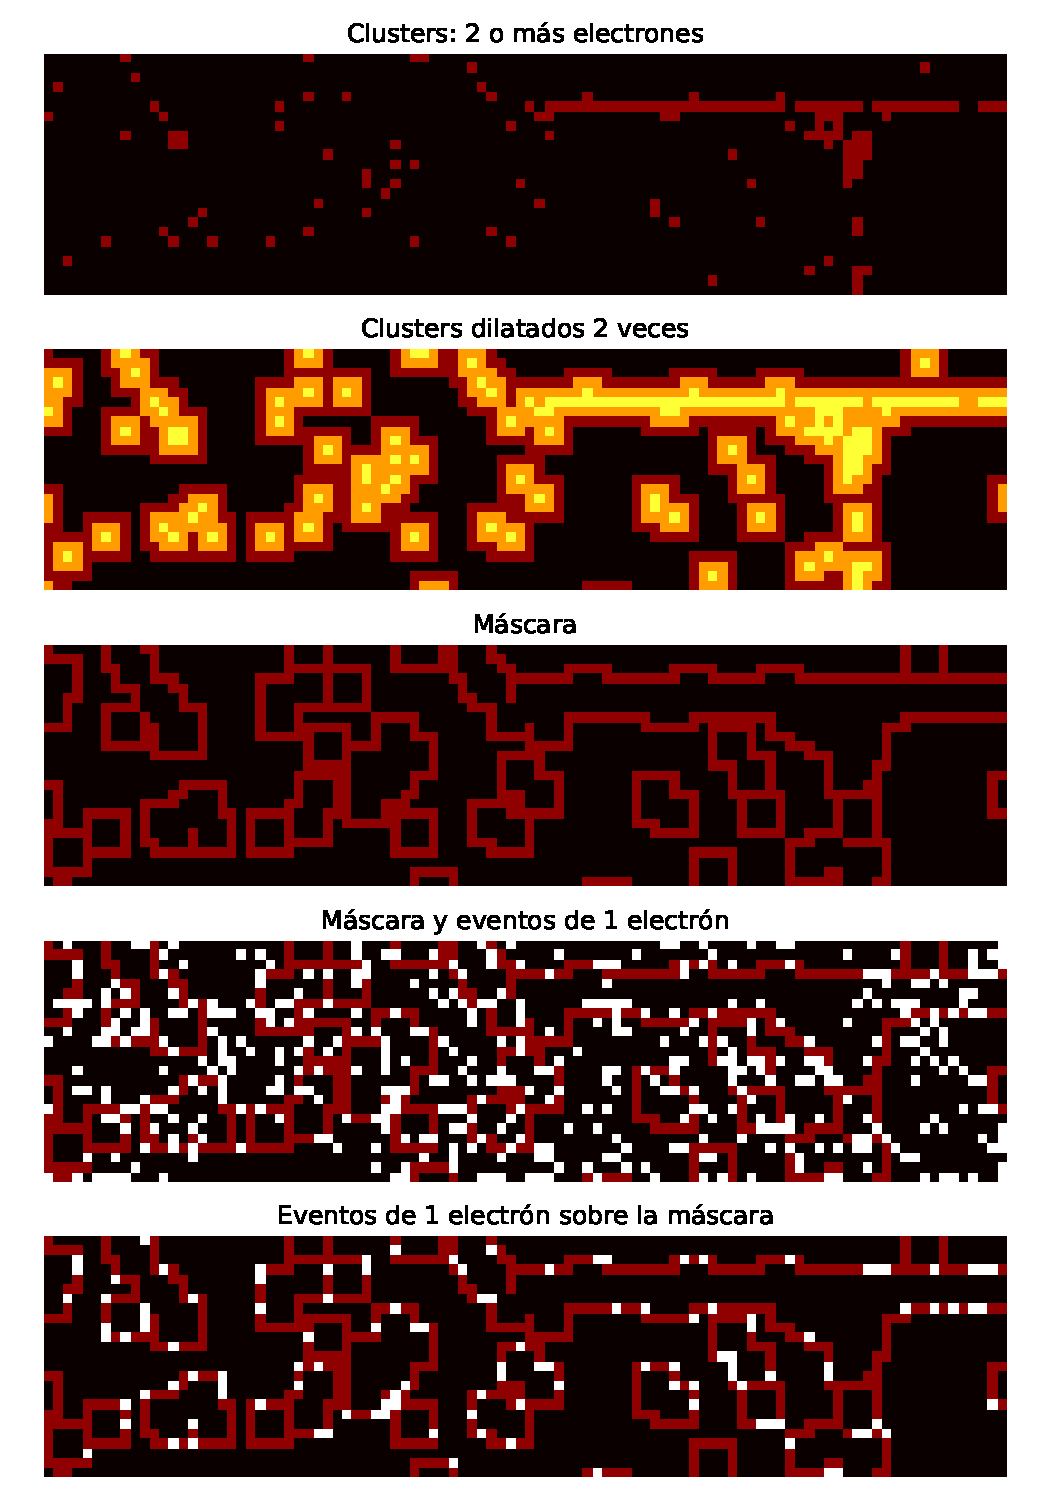
\includegraphics[scale=0.7]{Figs/analisis_bordesx2.pdf}
    \caption{\footnotesize{Análoga a la figura \ref{fig:AnalisisBordes}, pero para el caso de $2$ dilataciones, de forma de generar una máscara en el segundo borde. Los pasos son los mismos antes descriptos. De este proceso se halla la esperanza $\mu_{bkg}$.}}
    \label{fig:AnalisisBordesx2}
\end{figure}
La razón por la cual se usan los eventos inmediatamente contiguos a los bordes de los clusters para calcular el $\mu_{T}$, es porque se puede decir con seguridad que es la única región del sensor donde coexisten ambas contribuciones: $\mu_{bkg}$ y $\mu_{g}$. Tanto los eventos de un electrón que realmente pertenecen a los clusters como los eventos de un electrón que son espurios. Por otro lado, la razón por la cual se estima $\mu_{bkg}$ del siguiente cordón ($2$ píxeles de distancia al borde del cluster) se debe a que en esa zona es seguro que no pueden haber eventos genuinos de un cluster (o al menos la probabilidad de que eso suceda ronda los $10^{-14}$).\\
\indent Finalmente, de realizar estos análisis se obtuvieron los valores para las esperanzas de ambas contribuciones, que resultaron ser:
\begin{equation*}
    \mu_{T} = 0.19735 \pm 0.00024
\end{equation*} 
y el valor de la esperanza para los eventos espurios resultó 
\begin{equation*}
    \mu_{bkg} = 0.18583 \pm 0.00021
\end{equation*}
con lo cual, la esperanza para los eventos genuinos es 
\begin{equation*}
    \mu_{g} = 0.011524 \pm 0.00031
\end{equation*}
Teniendo estos valores puede corregirse el conteo de carga en los clusteres, tanto por exceso como por defecto y así tener una medición más precisa del factor de Fano y la energía de creación electrón-hueco.

\subsection{Corrección del conteo de carga}
\noindent El punto de todo el análisis anterior era poder generar las herramientas para corregir el conteo de carga que hace el programa de detección de clusters, luego de aplicar un umbral que podría eliminar carga genuina y, además, poder estimar cuánta carga excedente proveniente de fondo tiene cada cluster.\\

Esta va toda nueva. No me queda claro como era la correción
%\indent Esta corrección se llevó a cabo modificando el código del programa que con \textit{Root} calcula el factor de Fano, la energía de creación electrón-hueco, y otras variables, por medio del ajuste de los espectros de carga. El programa se encarga de procesar todas las imágenes, desechar eventos que tengan carga menor a $2$ electrones (\verb|EPIX = 1.5|), filtrar eventos que no cumplan ciertos criterios (cortes de calidad), buscar los clusters, quedarse únicamente con aquellos que tengan cargas en el entorno de los $180$ electrones y calcular esos valores. Al contar la carga de estos clusters y conociendo el área de los mismos (cantidad de píxeles que los conforman), se agrega y se quita carga en función de los valores hallados antes.\\
%\indent Dado que la distribución de la variable aleatoria \textit{cantidad de eventos por píxel} sigue una distribución poissoniana, de esperanza $\mu$, para cada tipo evento (espurio, genuino o total) se tiene una esperanza. Para calcular la cantidad de carga que se espera que tenga un cluster de $N$ píxeles en el sensor, se puede hacer uso de las propiedades de la esperanza. Sea $Y = \sum\limits_{i = 1}^{N} X_{i}$, donde $X_{i}$ son distintas realizaciones de la variable aleatoria con distribución Poissoniana y $N$ es el número de píxeles del cluster, entonces la esperanza se calcula como
% \begin{equation*}
%     E(Y) = 
%     E
%     \left(
%         \sum\limits_{i=1}^{N} X_{i}
%     \right)
%     = \sum\limits_{i=1}^{N}E(X_{i})
%     = \sum\limits_{i=1}^{N}\mu_{i}
%\end{equation*}
%pero como $X_{i}$ son distintas realizaciones de la misma variable aleatoria, entonces tienen todas la misma esperanza, es decir $\mu_{i} = \mu\ \forall\ i$, con lo cual
%\begin{equation*}
%    E(Y) = N\mu
%\end{equation*}
%con lo cual, la cantidad de carga esperada para un cluster viene dada por la esperanza de la distribución, por la cantidad de píxeles. De esta forma, teniendo una esperanza total $\mu_{T} = \mu_{bgk} + \mu_{g}$, aplicando esta misma receta pueden corregirse los valores de carga por cluster. Si $n_{e}$ es la cantidad de carga medida en un dado cluster, la corrección de este valor de carga será $n_{c}$ y viene dado por
%\begin{equation*}
%    n_{c} = n_{e} + N\mu_{g} - N\mu_{bkg}
%\end{equation*}
%es decir, se agrega la cantidad de carga que se estima se pierde en los bordes por aplicar el umbral \verb|EPIX = 1.5| y se quita la carga estimada por ruido en el interior de los clusters. \textcolor{red}{Acá no me queda del todo claro como era el tema del redondeo: $N\mu_{g}$ y $N\mu_{bkg}$ claramente son float, pero la carga tiene que ser entera. El redondeo donde se hacía?}
